\documentclass[11pt,reqno]{amsart}
\usepackage[parfill]{parskip}
\usepackage{graphicx}

\usepackage{epstopdf}
\usepackage{enumerate}
\usepackage{sgame}

\usepackage[dvipsnames,table]{xcolor}
\usepackage{colortbl}

\usepackage{tikz}
\usepackage{pgfplots}
\pgfplotsset{compat=1.12}

\usepackage{amssymb}
\usepackage{bbm}
%\usepackage[urw-garamond]{mathdesign}
%\usepackage{nomencl}
\usepackage[type1]{libertine}
\usepackage[T1]{fontenc}
\usepackage[libertine]{newtxmath}
\usepackage{dsfont}
%\usepackage{classico}
%\usepackage{merriweather}

%\usepackage[T1]{fontenc}
%\usepackage{stix}




\usepackage{rotating}
\usepackage{booktabs}


\usepackage[margin=0.8in]{geometry}


\usepackage{graphicx} % support the \includegraphics command and options

% \usepackage[parfill]{parskip} % Activate to begin paragraphs with an empty line rather than an indent


%\DeclareSymbolFont{cmlargesymbols}{OMX}{cmex}{m}{n}
%\let\sum\relax
%\DeclareMathSymbol{\sum}{\mathop}{cmlargesymbols}{"50}
%
%\DeclareSymbolFont{cmlargesymbols}{OMX}{cmex}{m}{n}
%\let\int\relax
%\DeclareMathSymbol{\int}{\mathop}{cmlargesymbols}{"52}


\newtheorem{theorem}{\textsc{Theorem}}
\newtheorem{definition}{\textsc{Definition}}
\newtheorem{proposition}{\textsc{Proposition}}

\renewcommand{\baselinestretch}{1.2}
%\setlength{\textwidth}{15cm}


\newcommand{\st}{\rho} %Probability of a given state of the environment (or game)
\newcommand{\ha}{h} %Information upon which an individual bases its updating of action values
\newcommand{\e}{\theta} %A state of the environment
\newcommand{\Et}{\Theta} %Set of states of the environment
\newcommand{\At}{V} %Action value at a given time 
\newcommand{\dAt}{\Delta\At} %Set of states of the environment
\newcommand{\na}{n} %Number of available actions
\newcommand{\ac}{a} %An action
\newcommand{\Ac}{\mathcal{A}} %Set of actions
\newcommand{\p}{p} %Probability that an individual takes a given action
\newcommand{\vp}{\mathbf{p}} %Vector of probabilities of taking actions
\newcommand{\de}{\mathop{}\!\mathrm{d}} %derivative
\newcommand{\va}{\mathbf{a}} %Vector of actions (or action profile) of all players in a game
\newcommand{\vm}{\mathbf{\At}} %Vector of action values for a player
\newcommand{\iv}{\mathds{1}} %Indicator variable
\newcommand{\Rp}{\mathcal{R}} %The four following parameters are the generic payoffs for a social dilemma
\newcommand{\Sp}{\mathcal{S}}
\newcommand{\Tp}{\mathcal{T}}
\newcommand{\Pp}{\mathcal{P}} 
\newcommand{\pay}{\pi} %Material payoff
\newcommand{\lr}{\gamma} %Learning rate in the stochastic approximation algorithm
\newcommand{\xr}{\xi} %Exploration parameter


\newcommand{\Esp}{\mathds{E}} %Expectation operator
\newcommand{\Prb}{\mathds{P}} %Probability
\newcommand{\Rn}{\mathds{R}} %The set of real numbers


\newcommand{\np}{N}%number of players
\newcommand{\tm}{t}%time index
\newcommand{\om}{o} %A game outcome
\newcommand{\Om}{\mathcal{O}} %Set of game outcomes
\newcommand{\fc}{f} %Fecundity function
\newcommand{\ru}{\ell} %Learning rule: function mapping the previous individual's state and new information, to a new individual's state
\newcommand{\pf}{u} %Utility of a player for a game outcome
\newcommand{\vpf}{\mathbf{u}} %Vector of utilities of a player in the discrete action model
\newcommand{\pft}{v} %Utility of a "second" player for a game outcome
\newcommand{\vpft}{\mathbf{v}} %Vector of utilities of a "second" player in the discrete action model
\newcommand{\Pf}{U} %Set of utility functions, where evolution takes place
\newcommand{\ma}{m} %Mean action of a player in the continuous action model
\newcommand{\sd}{\sigma} %Standard deviation of the action of a player in the continuous action model
\newcommand{\Nd}{\mathcal{N}} %Normal distribution
\newcommand{\vma}{\boldsymbol{\ma}} %Vector of mean action of all players in the continuous action model
\newcommand{\rf}{R} %Reward to an action in the continuous action model
\newcommand{\vrf}{\mathbf{\rf}} %Vector of rewards to an action in the continuous action model
\newcommand{\pd}{\partial}
\newcommand{\Hs}{\mathbf{H}} %Hessian matrix
\newcommand{\var}{\mathrm{Var}}
\newcommand{\cov}{\mathrm{Cov}}
\newcommand{\mx}{M} %
\newcommand{\dv}{\delta} %Deviation of a mutant from the resident phenotype
\newcommand{\vd}{\boldsymbol{\dv}}
\newcommand{\ba}{\beta} %Best (NE) action in the one-player continuous game
\newcommand{\bn}{b} %Benefit of cooperation
\newcommand{\cs}{c} %Cost of cooperation
\newcommand{\vh}{k} %Factor of proportionality between the value of the hare and the stag in the Stag hunt game
\newcommand{\lp}{q} %Lock-in probability
\newcommand{\Rs}{\textrm{R}} %Lock-in probability
\newcommand{\eg}{\lambda} %eigenvalue
\newcommand{\sgn}{\textrm{sign}} %eigenvalue



\title[Preferences and learning]{Evolution of rewards in games}
\date{\today}

\begin{document}
\maketitle





\section{Introduction}

This is an introduction to the paper.

\section{Model}


\subsection{Game, payoffs, and utilities}


We consider a general $\np$-player game where each player $i$ has an action set $\Ac_i$ from which it can choose an action $\ac_i \in \Ac_i$. We think of these $\np$ players as belonging to a larger population, where a (random) matching has occurred between population members that generated many groups of $\np$ players (see below the evolutionary setting). The action space $\Ac_i$ can be a finite set of $\na$ discrete actions or a continuous set, such as a subset of $\Rn$. The environment as well as the actions of the other players affect the material payoff of every individual. There is a set $\Et$ of environmental states, with typical element $\e\in\Et$ (the environment can also be continuous or discrete). The material payoff of a player is given by the function $\pay_i : \prod_{j\in \np} \Ac_j \times \Et  \to \Rn$, which ultimately affects the fitness of $i$ (see below for details). To simplify notation, we will also write $\Ac = \prod_{j\in \np} \Ac_j$ for the set of all possible action profiles.

The players have subjective preference or utility functions, $\pf_i : \prod_{j\in \np} \Ac_j \times \Et  \to \Rn$, that may differ from the objective material payoff $\pay_i$. The utility function $\pf_i$ is genetically determined and is the evolving trait: we are interested in the function(s) $\pf_i$ that is(are) favored by natural selection. In the forthcoming analysis of the model, it may be easier to think of the game as having a single-valued ``outcome'', $\om$ that is a function of the action profile and the environment, i.e.~$\om(\va,\e)\in \Om$, where the outcome space, $\Om$, is a subset of $\Rn$. The utility function may then be defined directly over outcomes $\pf_i : \Om  \to \Rn$.

The game is repeated at discrete times $\tm = 1,2,\dots$ and the players choose an action profile $\va_\tm$. The environment fluctuates independently from the players' actions and takes value $\e_\tm$ at time $\tm$. The probability that state $\e$ occurs at time $\tm$ is written $\st(\e)$, and is thus independent of time (i.i.d. environment). The players cannot observe the state of the environment prior to choosing their actions. The material payoff to player $i$ when the action profile is $\va_\tm$ and the environment is in state $\e_\tm$ is given by $\pay_i(\va_\tm,\e_\tm)$, which we may also write $\pay_i(\ac_{i,t}, \va_{-i,t},\e_\tm)$, where $\va_{-i,t} \in \prod_{\substack{j\in \np \\ j\neq i}} \Ac_j$ is the action profile of all players except player $i$. Each individual observes privately the utility $\pf_i(\va_\tm,\e_\tm)$ which results from the game outcome $\om_\tm = (\va_\tm,\e_\tm)$ at time $\tm$.



\subsection{Learning}

The learning model is taken from Dridi \& Lehmann (2014), where players use the material payoffs of the game to update motivations about actions. Our learning model will not be very different from this previous work because all we have to change is that individuals update their choice probabilities using the subjective utility of a game outcome, rather than the objective material payoff. Hence, the difference between this previous paper and our formulation of learning dynamics is that in Dridi \& Lehmann (2014), the games considered are symmetric, while here the utility function of each player is different, which translates into an asymmetric game defined by the family of utility functions $(\pf_i)_{i\in \np}$.

While the general model of Dridi \& Lehmann (2014) allows for both trial-and-error learning and belief-based learning, we will first only consider trial-and-error learning. At every time $\tm$ of the repeated game defined above, each individual $i$ holds in memory action values $\At_{i,\tm}(\ac_i)$ for all actions $\ac_i \in \Ac_i$. The learning rule of individual $i$ is to update action values according to
\begin{equation}
\label{Lrule}
\At_{i,\tm+1}(\ac_i) = \At_{i,\tm}(\ac_i) + \lr_\tm  \iv(\ac_i,\ac_{i,\tm}) \pf_{i}(\ac_i,\va_{-i,\tm},\e_\tm),
\end{equation} 
where $\lr_\tm \in (0,1)$ is a decreasing learning rate in the sense of stochastic approximation theory. This decreasing learning rate allows us to approximate the above stochastic difference equation with a deterministic mean-field differential equation that asymptotically tracks the original stochastic dynamics. The expression $\iv(\ac_i,\ac_{i,\tm})$ is an indicator variable that equals 1 if $\ac_i = \ac_{i,\tm}$, and 0 otherwise. While eq.~\ref{Lrule} is not very often used in the literature, it can be seen as a conscious updating of action values because an action that is not played at time $\tm$ keeps the same action value at time $\tm+1$. Traditionally in reinforcement learning models, actions that are not played for a long period of time tend to be forgotten, and hence their values come back to 0. Our model captures more learning processes where early experience is critical in determining stable outcomes, and hence may be used to capture fast learning dynamics rather than lifelong learning processes.

We generally call the right-hand side of eq.~\ref{Lrule} the learning rule, written $\ru_i(\At_{i}, h_i)$, of individual $i$. The learning rule takes the previous vector of action values $\At_{i}$ and a new information $h_i$ (in our present model, $h_i = \pf_{i}(\cdot,\va_{-i,\tm},\e_\tm)$, but one could think of more general updating rules) and outputs a new vector of action values. Player $i$ chooses an action $\ac_{i,\tm}$ at time $\tm$ with a probability that depends on its action values $\At_{i,\tm} = \{ \At_{i,\tm}(\ac_i) \}_{\ac_i\in\Ac_i}$. One possibility is to assume a perturbed maximization scheme which gives rise to the logit-choice function,
\begin{equation}
\label{logitchoice}
\p_{i,t}(\ac_i) = \frac{\exp[\xr \At_{i,t}(\ac_i)]}{\sum_{b_i\in \Ac_i} \exp[\xr \At_{i,t}(b_i)]},
\end{equation}
where $\xr$ is the exploration parameter (the inverse $1/\xr$ can be seen as the noise level) in choosing actions. We write $\p_{i,t}$ without the action argument to denote the whole vector of action probabilities of player $i$.


\section{Fecundity}

We define the total payoff of individual $i$ as the average material payoff obtained at equilibrium of the learning process, i.e.
\begin{equation}
\label{fec}
\fc_{i} = \fc(\pf_i) = \int_{\Ac} \sum_{\e\in\Et} \hat{\vp}(\va) \st(\e) \pay_i(\va,\e) \de \va,
\end{equation}
where $\hat{\vp}(\va) = \prod_{j\in N} \hat{\p}_j(\ac_j)$ is the equilibrium probability of action profile $\va = (\ac_1,\dots,\ac_\np)$. This is the product of individuals' equilibrium action probabilities $\hat{\p}_j(\ac_j)$. (In the continuous action setting, we always assume that the probability distribution over actions admits a density). Importantly, while the utility function does not appear on the rhs of eq.~\ref{fec}, we still defined it as $\fc(\pf_i)$ because the equilibrium choice probabilities of a player, $\hat{\p}_i(\ac_i)$, implicitly depend on the utility function of player $i$.

\section{Preference evolution and the set of possible utility functions}

Consider a very large population and assume that groups of $\np$ players are randomly formed at every generation to play the above repeated game. An individual's genotype corresponds to its utility function $\pf_i(\cdot)$, which he transmits to its offspring. The number of offspring he produces depends on its material payoffs obtained during the game as defined in eq.~\ref{fec}. In the most general case, the set in which evolution occurs is the set of all possible utility functions $\pf : \prod_{j\in \np} \Ac_j \times \Et  \to \Rn$. Let $\Pf$ denote such a set. When the action space is discrete, the space of utility functions is $\Rn^{|\Om|}$, where $\Om = \prod_{j\in \np} \Ac_j$ is the set of possible game outcomes. Hence the dimension of the state space is equal to $|\Om| = \prod_{j\in \np} |\Ac_j|$. In a symmetric game where all $\np$ players have $\na$ actions, the dimension of $\Pf$ is thus equal to $|\Om| = \na^\np$.


\section{Symmetric two-player games}

In this section we consider a reduction of the model for symmetric constant two-player games. The action set for each player $i$ is $\Ac_{i} = \{ 1,2 \}$, where we identify action 1 with cooperation, and action 2 with defection.


\subsection{Four-dimensional adaptive dynamics}

The set $\Pf$ consists of all possible $2\times 2$ real matrices, which can be identified with the set $\Rn^{2\times 2}=\Rn^4$. The genotype of an individual can thus also be seen as the vector $\vpf = (\pf_{11},\pf_{12},\pf_{21},\pf_{22})$, where $\pf_{ij}$ denotes the utility to the focal individual when he chooses action $i$ and his opponent chooses action $j$.

With such definitions, one can use standard approaches in evolutionary biology, such as adaptive dynamics, in order to find the ESS utility matrix, and the analysis can be complemented to look at convergence stability. Under this approach one considers a resident population with utility $\vpf$ and asks whether a mutant with utility $\vpf+\vd$ can invade or not. One advantage of this approach in our learning context is that the ``utility game'' between the resident and the mutant is quasi-symmetric, which implies that the learning dynamics determining behavior is a family of dynamics for quasi-symmetric games. This is a substantial simplification of the analysis. Save the bifurcations, the quasi-symmetric game between $\vpf$ and $\vpf+\vd$ is very close to the symmetric game defined by $\vpf$, because the vector field determining the learning dynamics is continuous in $\vpf$.

A candidate ESS is such that
\begin{equation}
\label{cES}
\left. \frac{\pd \fc}{\pd \vpf}\right|_{\vpf=\vpf^*} = 0.
\end{equation}
Even before embarking on the analysis of eqs.~\ref{fec}--\ref{cES}, one can remark that it is not certain that a unique strategy $\vpf^*$ can be found using standard maximization approaches. Indeed, there are discontinuities in $\fc$ occurring when at least one utility changes sign. This is because $\fc$ depends on the dynamical system describing the behavioral interactions between learners in the population. The behavioral dynamics actually changes completely (i.e. stable equilibria appear/disappear) when a utility changes sign, which means that there are bifurcations at the 0 axes (when $\pf_{ij}=0$). In order to perform a full analysis of the model, one has to deal with the bifurcations occurring when at least when utility changes sign. These complications are best illustrated in the simplified model that we study below.





\subsection{Analysis of the behavioral interactions between the strategies}


\subsubsection{Generic analysis of a 2-player interaction}

In order to compute fitness for a player, one needs to predict the outcome of behavioral interactions when this player is matched with another player that has a different utility function. The behavioral interaction between a reinforcement learner with utilities $\vpf = (\pf_{11},\pf_{12},\pf_{21},\pf_{22})$ and another reinforcement learner with utilities $\vpft = (\pft_{11},\pft_{12},\pft_{21},\pft_{22})$ determines a dynamical system in $[0,1]^2$. By a slight abuse of notation, let denote these two players $\pf$ and $\pft$ and their probabilities to cooperate by $\p_{\pf}$ and $\p_{\pft}$ respectively. The utilities $\vpf$ and $\vpft$ themselves define an asymmetric 2-player game:
\begin{equation}
\label{prefMat}
\left[ \begin{array}{cc}
    (\pf_{11}, \pft_{11}) & (\pf_{12}, \pft_{21})  \\ 
    (\pf_{21}, \pft_{12}) & (\pf_{22}, \pft_{22})  \\ 
  \end{array}  \right],
\end{equation}
where player $\pf$ chooses a row and player $\pft$ chooses a column. Remark that the notation for utilities are player-centered: $x_{ij}$ is the utility to player $x$ when he plays $i$ and his opponent plays $j$. However, when we refer to an outcome of the game without explicitly mentioning the players, we write it in the form $(\ac_\pf, \ac_\pft)$, treating player $\pf$ as the default focal player. Analyzing a generic behavioral interaction between two reinforcement learners with arbitrary utilities amounts to analyzing the behavioral dynamics of reinforcement learning in arbitrary two-player asymmetric games.

Using stochastic approximation theory, one obtains a system of differential equations describing the long-run dynamics of eqs.~\ref{Lrule}--\ref{logitchoice}, which reads
\begin{align}
\label{dynotwoRM}
 \dot{\p}_u  &=  \p_u(1-\p_u) \xr \left[ \p_u  \{\p_v \pf_{11}+(1-\p_v)\pf_{12}\}  - (1-\p_u) \{\p_v \pf_{21}+(1-\p_v)\pf_{22}\}  \right], \nonumber \\
 \dot{\p}_v  &=  \p_v(1-\p_v) \xr \left[ \p_v \{\p_u \pft_{11}+(1-\p_u)\pft_{12}\}  - (1-\p_v) \{\p_u \pft_{21}+(1-\p_u)\pft_{22}\}  \right].
\end{align}
In Fig.~\ref{genBeh}, we show the ten possible equilibria of eq.~\ref{dynotwoRM}. We call these the generic behavioral equilibria. Depending on the specific values of $\vpf$ and $\vpft$, some of these equilibria may not exist anymore.


The sign of the utilities $\vpf$ and $\vpft$ play a fundamental role in determining the stability of the different behavioral equilibria. Indeed, one has that a pure equilibrium is locally stable if and only if both players have a positive utility for this outcome. In other words, if players $\pf$ and $\pft$ do not ``agree'' on preferred outcomes, then a pure behavioral equilibrium cannot be stable. This intuitive result is mathematically true because the eigenvalues of the Jacobian matrix evaluated at a pure outcome $(i,j)$ are simply
\begin{equation}
\eg_1 = -\xr \pf_{ij}, \eg_2 = -\xr \pft_{ji}.
\end{equation}
This has important evolutionary consequences. Under the assumption that fitness is evaluated only at equilibrium of the learning process, it means that as long as two strategies have utilities of the same signs, none has an evolutionary advantage over the other (except for strategies in the ``Mismatcher'' class, $\sgn(\vpf) = (-,+,-,+)$, or ``Reluctant'' strategies, $\sgn(\vpf) = (-,-,-,-)$).  
Mixed behavioral equilibria (i.e., equilibria where at least one player has a mixed strategy) require a little more work. First one notices that the four mixed equilibria on the boundaries exist only if the utilities of the mixing player have the same sign. For instance, the equilibrium $\left(\frac{\pf_{21}}{\pf_{11} + \pf_{21}},1\right)$ on the top boundary of the state space exists only when $\pf_{11}$ and $\pf_{21}$ have the same sign.

%TO DO: I CAN DO MORE IN TERMS OF THE GENERIC ANALYSIS OF A BEHAVIORAL INTERACTION, BECAUSE THE SIGN OF THE EIGENVALUES ASSOCIATED WITH EQUILIBRIA DEPENDS ON RATHER SIMPLE INEQUALITIES, INVOLVING THE UTILITIES OF BOTH PLAYERS. THIS IS IN THE SAGE NOTEBOOK







\subsubsection{Subset of strategies}


In this section we calculate the payoffs and fitnesses for all possible behavioral interactions between the 4 strategies Realistic, Other-regard, Selfish, and Manipulator. From these calculations, we derive invasion conditions within this set of strategies.

Some assumptions need to be made in order to compute analytical expressions for long-term payoffs. First, when the behavioral dynamics admit several stable equilibria, typically the stochastic dynamics may converge to any of these stable equilibria. It may not always be possible to know which particular equilibrium will be reached by the stochastic process, because the trajectory may go out from the basin of attraction of a stable equilibrium under the influence of large stochastic shocks (these large shocks are more likely to occur at the beginning of a behavioral interaction). For these reasons, we assume that the initial preferences of players are unbiased, such that the process starts in the center of the state space ($\p_1 = \p_2 = 1/2$). Also, we assume that the process may reach each equilibrium with equal probability; in other words, the distribution of stable equilibria is uniform. Such an assumption is valid for relatively high values of the exploration rate, $\xr\approx 10$ (Dridi \& Lehmann, 2015).






%\clearpage









%\begin{table}[]
%\tiny
%\caption{Classification of behavioral outcomes and resulting fitness in the discrete action model amongst the 4 strategies considered.}
%\label{behOut}
%\begin{sideways}
%\rowcolors{2}{gray!25}{white}
%\begin{tabular}{@{}llllllll@{}}
%\toprule
%        & Always stable equilibria                       & Sometimes stable equilibria                                               & Stability condition                           & Generic fitness                                                                                                                                                                                                                                                 & Fitness in PD & Fitness in SH & Fitness in SD \\ \midrule
%R vs.~R &                                                &                                                                           &                                               &                                                                                                                                                                                                                                                                 &               &               &               \\ \midrule
%R vs.~A & $(0,0)$ and $(1,1)$                            &                                                                           &                                               & $(\frac{1}{2}\Rp, \frac{1}{2}\Rp)$                                                                                                                                                                                                                              &               &               &               \\ \midrule
%R vs.~P & $(1,1)$ and $(0,\frac{v_{22}}{v_{12}+v_{22}})$ &                                                                           &                                               & $(\frac{1}{2}\Rp, \frac{1}{2}\Rp)$                                                                                                                                                                                                                              &               &               &               \\ \midrule
%R vs.~O & $(0,1)$ and $(1,1)$                            &                                                                           &                                               & $(\frac{1}{2}(\Rp+\Tp), \frac{1}{2}(\Rp+\Sp))$                                                                                                                                                                                                                  &               &               &               \\ \midrule
%R vs.~M & $(1,1)$ and $(0,\frac{v_{22}}{v_{12}+v_{22}})$ &                                                                           &                                               & $\left(\frac{1}{2}\left(\Rp+\Tp\left(\frac{v_{22}}{v_{12}+v_{22}}\right)+\Pp\left(1-\frac{v_{22}}{v_{12}+v_{22}}\right)\right), \frac{1}{2}\left(\Rp+\Sp\left(\frac{v_{22}}{v_{12}+v_{22}}\right)+\Pp\left(1-\frac{v_{22}}{v_{12}+v_{22}}\right)\right)\right)$ &               &               &               \\ \midrule
%R vs.~S & $(0,0)$                                        &                                                                           &                                               & $(\Pp, \Pp)$                                                                                                                                                                                                                                                    &               &               &               \\ \midrule
%O vs.~O & $(1,1)$                                        &                                                                           &                                               & $(\Rp, \Rp)$                                                                                                                                                                                                                                                    &               &               &               \\ \midrule
%O vs.~M & $(1,0)$ and $(1,1)$                            &                                                                           &                                               & $(\frac{1}{2}(\Rp+\Sp),\frac{1}{2}(\Rp+\Tp),)$                                                                                                                                                                                                                  &               &               &               \\ \midrule
%O vs.~S & $(1,0)$                                        &                                                                           &                                               & $(\Sp, \Tp)$                                                                                                                                                                                                                                                    &               &               &               \\ \midrule
%M vs.~M & $(1,1)$                                        & $(\frac{u_{22}}{u_{12}+u_{22}},0)$ and $(0,\frac{v_{22}}{v_{12}+v_{22}})$ & $|u_{12}| < |u_{21}|$, $|v_{12}| < |v_{21}|$, & $(\Rp,\Rp)$ or ...                                                                                                                                                                                                                                              &               &               &               \\ \midrule
%M vs.~S & $(\frac{u_{22}}{u_{12}+u_{22}},0)$             &                                                                           &                                               & $\left(\Sp\left(\frac{u_{22}}{u_{12}+u_{22}}\right)+\Pp\left(1-\frac{u_{22}}{u_{12}+u_{22}}\right),\Tp\left(\frac{u_{22}}{u_{12}+u_{22}}\right)+\Pp\left(1-\frac{u_{22}}{u_{12}+u_{22}}\right)\right)$                                                          &               &               &               \\ \midrule
%S vs.~S & $(0,0)$                                        &                                                                           &                                               & $(\Pp, \Pp)$                                                                                                                                                                                                                                                    &               &               &               \\ \bottomrule
%\end{tabular}
%\end{sideways}
%\end{table}







%\begin{figure}[htb]
%\begin{center}
%\begin{game}{2}{2}
%& & \\
%& {$+$} &$-$\\
%&$-$&$-$\\
%\end{game}
%
%Test
%\caption[]{A game with a colored cell.}\label{f:coloredCell}
%\end{center}
%\end{figure}

%\subsection{Constant public-goods games}
%
%If we let $\om$ be the total benefit produced in a public-goods game, then we may look for utility functions defined over this outcome.
%
%\subsection{Nash demand game}
%








\clearpage


\section{Continuous action space}

\subsection{Normally distributed actions}

Here, we treat the case where the action space is one-dimensional continuous, e.g., when $\Ac_i \subseteq \Rn$ for all $i$. This allows to capture investment games such as a continuous public goods game. We adapt a model of Beigy \& Meibody (2006), who study learning of a single decision-maker who faces a stochastic stationary environment. In their setting, the decision-maker tries to minimize the expectation of a given cost function where at each discrete time step he can exert an action $\ac \in \Rn$. In order to adapt their model to multi-player games, only a few tweaks need to be made.

We consider that at each time step $\tm$, every player is characterized by a mean action $\ma_{i,\tm}$, and a standard deviation $\sd_{i,\tm}$. The action $\ac_{i,\tm}$ chosen by $i$ at time $\tm$ is then drawn from a normal distribution with mean $\ma_{i,\tm}$ and standard deviation $\sd_{i,\tm}$, i.e., $\ac_{i,\tm} \sim \Nd(\ma_{i,\tm},\sd_{i,\tm})$. A possible interpretation of this model of action choice is that $\ma_{i,\tm}$ represents the preferred action by player $i$, which he would like to implement but there is a stochastic perturbation during action choice, such that $\ac_{i,\tm} = \ma_{i,\tm} + \varepsilon_{i,\tm}$, where $\varepsilon_{i,\tm} \sim \Nd(0,\sd_{i,\tm})$ is independent across players and time steps. With this interpretation, $\varepsilon_{i,\tm}$ can be seen as an exogenous noise during action implementation, or can also be seen as explicit exploration of the player around its preferred action (note that this model of action perturbation is different from the above model of payoff perturbation that generates the logit choice rule, eq.~\ref{logitchoice}).

Since a normal distribution is fully specified by its mean and standard deviation, in order to know the action distribution of a player at time $\tm+1$, we only need to know how $\ma_{i,\tm+1}$ and $\sd_{i,\tm+1}$ are updated given the previous values at time $\tm$ and the outcome of the game. We will use the following updating rule for the mean action,
\begin{equation}
\label{upCa}
\ma_{i,\tm+1} = \ma_{i,\tm} + \lr_\tm \pf_{i}(\ac_{i,\tm},\va_{-i,\tm},\e_\tm) \left( \frac{\ac_{i,\tm}- \ma_{i,\tm}}{\sd_{i,\tm}} \right),
\end{equation}
which essentially entails that the individual wants his new mean action $\ma_{i,\tm+1}$ to come closer to the chosen action $\ac_{i,\tm}$ if the obtained utility $\pf_{i}(\ac_{i,\tm},\va_{-i,\tm},\e_\tm)$ is positive, while he wants his mean action to move away from $\ac_{i,\tm}$ if the obtained utility is negative; the magnitude of such movement is proportional to the actual magnitude of the obtained utility. Consequently, this is one of the simplest way of capturing in a continuous action setting the biological notion of approach towards rewards and avoidance of punishments. %This thus implies that there is an increase in the mean action if the obtained utility $\pf_{i}(\ac_{i,\tm},\va_{-i,\tm},\e_\tm)$ and the difference $\ac_{i,\tm}- \ma_{i,\tm}$ have the same sign. Conversely, there is a decrease in the mean action if the obtained utility $\pf_{i}(\ac_{i,\tm},\va_{-i,\tm},\e_\tm)$ and the difference $\ac_{i,\tm}- \ma_{i,\tm}$ have opposite sign.
The standard deviation $\sd_{i,\tm}$ appears in the denominator of the reinforcement in eq.~\ref{upCa} so that the individual accounts for its own exploration strategy when updating action value: if $\sd_{i,\tm}$ is large, then there is a large probability that $\ac_{i,\tm}$ will be far from the mean, so the utility obtained by the individual should not be interpreted as reflecting a wrong mean action $\ma_{i,\tm}$ (the utility is mainly a reflection of the great variance in action choice), hence the update should be minor. Finally, the learning rate $\lr_\tm$ must obey the assumptions of stochastic approximation theory, just as in the discrete-action model (eq.~\ref{Lrule}) in order to ensure convergence of the learning process.

In the case where $\sd_{i,\tm} = \sd_{i}$ is a constant, independent of time, then  $\sd_{i}$ acts as an additional learning rate, that scales the speed at which the mean-field deterministic dynamics converge to an equilibrium: larger variance should lead to faster convergence (see the analysis below for details).

A technical assumption needed to make the analysis tractable is that $\pf_{i}(\ac_{i,\tm},\va_{-i,\tm},\e_\tm)$ is twice continuously differentiable in the actions of all the players (note that this may create some problems when defining games with bounded action space, where typically the payoff function is not differentiable on the boundaries).

The vector $\vma_\tm = (\ma_{1,\tm},\dots,\ma_{\np,\tm})$ collects the mean action of all players at time $\tm$.


\subsection{Stochastic approximation}

Let $\rf_{i,t+1} = \pf_{i}(\ac_{i,\tm},\va_{-i,\tm},\e_\tm) \left( \frac{\ac_{i,\tm}- \ma_{i,\tm}}{\sd_{i,\tm}} \right)$ be the reinforcement to the mean action of player $i$, and let $\vrf_{\tm+1} = (\rf_{i,\tm+1})_{i\in\np}$ denote the vector collecting the reinforcements of all the players at time $\tm+1$. Stochastic approximation theory tells us that $\Esp[\vrf_{t+1} | \vma_\tm]$ is a vector field that defines a differential equation for $\vma$ whose asymptotic path is followed by the original stochastic process $\{ \vma_\tm \}_{t\geq 0}$. To obtain an explicit expression for $\Esp[\vrf_{t+1} | \vma_\tm]$, we use a second-order Taylor series expansion of $\pf_{i}(\ac_{i,\tm},\va_{-i,\tm},\e_\tm)$ around $\ma_{i,\tm}$, which gives
\begin{multline}
\label{RfExp}
\Esp[\rf_{i,t+1} | \vma_\tm] =  \Esp \Big[ \Big(\pf_{i}(\ma_{i,\tm},\vma_{-i,\tm},\e_\tm) + \nabla \pf_{i}(\ma_{i,\tm},\vma_{-i,\tm},\e_\tm)^{\textrm{T}} (\va_\tm  - \vma_\tm) \\
 + (\va_\tm  - \vma_\tm)^{\textrm{T}} \Hs \pf_{i}(\ma_{i,\tm},\vma_{-i,\tm},\e_\tm) (\va_\tm  - \vma_\tm) \Big) \frac{(\ac_{i,\tm}- \ma_{i,\tm})}{\sd_{i}} \Big| \vma_\tm \Big],
\end{multline}
where $\nabla \pf_{i}(\ma_{i,\tm},\vma_{-i,\tm},\e_\tm) = \left(\frac{\pd \pf_{i}}{\pd \ma_{1,\tm}},\dots,\frac{\pd \pf_{i}}{\pd \ma_{\np,\tm}}\right)$ is the gradient vector and $\Hs \pf_{i}(\ma_{i,\tm},\vma_{-i,\tm},\e_\tm)$ is the Hessian matrix of $\pf_{i}$, with typical element $[\Hs \pf_{i}]_{kj} = \frac{\pd^2 \pf_{i}}{\pd \ma_{k,\tm} \pd \ma_{j,\tm}}$. The vector $\va_\tm  - \vma_\tm$ has typical element $\ac_{j,\tm}- \ma_{j,\tm}$. Taking the non-random terms out of the expectation, the above equation can be rewritten as
\begin{multline}
\label{RfExp2}
\Esp[\rf_{i,t+1} | \vma_\tm] = \frac{1}{\sd_{i}} \pf_{i}(\ma_{i,\tm},\vma_{-i,\tm},\e_\tm) \Esp \Big[ (\ac_{i,\tm}- \ma_{i,\tm}) \Big| \vma_\tm \Big] + \nabla \pf_{i}(\ma_{i,\tm},\vma_{-i,\tm},\e_\tm) \Esp \Big[ (\ac_{i,\tm}- \ma_{i,\tm}) (\va_\tm  - \vma_\tm) \Big| \vma_\tm \Big] \\
+ \Esp \Big[ (\ac_{i,\tm}- \ma_{i,\tm}) (\va_\tm  - \vma_\tm)^{\textrm{T}} \Hs \pf_{i}(\ma_{i,\tm},\vma_{-i,\tm},\e_\tm) (\va_\tm  - \vma_\tm) \Big| \vma_\tm \Big].
\end{multline}
In order to find expressions for the various expectations above it will be useful to keep in mind that for each player $i$, the random variable $\ac_{i,\tm}- \ma_{i,\tm}=\varepsilon_{i,t}$ is normally distributed with zero mean and variance $\sd_{i}^2$. In particular, this implies that $\Esp \Big[ (\ac_{i,\tm}- \ma_{i,\tm}) \Big| \vma_\tm \Big] = 0$ for all $i$, so that $\Esp \Big[ (\va_\tm  - \vma_\tm) \Big| \vma_\tm \Big] = (0, 0, \dots,0)$. Also
\begin{align}
\label{RfExp3}
\Esp \Big[ (\ac_{i,\tm}- \ma_{i,\tm}) (\va_\tm  - \vma_\tm) \Big| \vma_\tm \Big] & = \Big( \cov[\ac_{1,\tm},\ac_{i,\tm} | \vma_\tm],\dots,\var[\ac_{i,\tm}| \vma_\tm] ,\dots, \cov[\ac_{\np,\tm},\ac_{i,\tm}| \vma_\tm] \Big) \nonumber\\ 
 & = \Big( 0,\dots,\sd_{i}^2,\dots, 0 \Big),
\end{align}
because action choice is independent across players. (An interesting note here on social learning is that if players copy each other then $\cov[\ac_{j,\tm},\ac_{i,\tm}| \vma_\tm]$ of players $i$ and $j$ may be different than 0, depending on whether they can copy one another.) The term involving the Hessian matrix has the form
\begin{multline}
\label{RfExpH}
\Esp \Big[ (\ac_{i,\tm}- \ma_{i,\tm}) (\va_\tm  - \vma_\tm)^{\textrm{T}} \Hs \pf_{i}(\ma_{i,\tm},\vma_{-i,\tm},\e_\tm) (\va_\tm  - \vma_\tm) \Big| \vma_\tm \Big] = \\
 \sum_{j\in\np} \sum_{k\in\np} \frac{\pd^2 \pf_{i}}{\pd \ma_{k,\tm} \pd \ma_{j,\tm}} \Esp \Big[ (\ac_{i,\tm}- \ma_{i,\tm}) (\ac_{j,\tm}- \ma_{j,\tm}) (\ac_{k,\tm}- \ma_{k,\tm}) \Big| \vma_\tm \Big],
\end{multline}
where the triplet covariance $\Esp \Big[ (\ac_{i,\tm}- \ma_{i,\tm}) (\ac_{j,\tm}- \ma_{j,\tm}) (\ac_{k,\tm}- \ma_{k,\tm}) \Big| \vma_\tm \Big] $ is zero again because action choice is independent across players whenever at least one of  $j\neq i$ or $k\neq i$ or $k\neq j$ is true. When $j=i$ and $k=i$, this triplet equals $\Esp \Big[ (\ac_{i,\tm}- \ma_{i,\tm})^3 \Big| \vma_\tm \Big]=0$ (because the odd moments of a centered Normal distribution are 0). Thus we have
\begin{equation}
\label{RfExpH2}
\Esp \Big[ (\ac_{i,\tm}- \ma_{i,\tm}) (\va_\tm  - \vma_\tm)^{\textrm{T}} \Hs \pf_{i}(\ma_{i,\tm},\vma_{-i,\tm},\e_\tm) (\va_\tm  - \vma_\tm) \Big| \vma_\tm \Big] = 0.
\end{equation}
Plugging back the expressions of these expectations in eq.~\ref{RfExp2}, the expected reinforcement of player $i$ takes the simple form
\begin{equation}
\label{RfExp}
\Esp[\rf_{i,t+1} | \vma_\tm] = \sd_{i}  \frac{\pd \pf_{i}(\ma_{i,\tm},\vma_{-i,\tm},\e_\tm)}{\pd \ma_{i,\tm}}.
\end{equation}
Thus, the differential equation
\begin{equation}
\label{meanF}
\frac{\de \ma_i}{\de \tm} \equiv \dot{\ma}_i = \sd_{i}  \frac{\pd \pf_{i}(\ma_{i},\vma_{-i},\e)}{\pd \ma_{i}}, \qquad i\in\np
\end{equation}
describes the long-run stochastic dynamics of the mean action of player $i$. Eq.~\ref{meanF} is a gradient dynamical system, where every player can be seen as maximizing his own utility function. In previous work, such gradient dynamics have been used as an \emph{ad hoc} model of learning dynamics. It is interesting that we recover this result by explictly modeling the stochastic learning dynamics.

A counterintuitive feature of eq.~\ref{meanF}, when we compare it to eq.~\ref{upCa}, is that according to eq.~\ref{meanF}, learning speed should increase with the standard deviation $\sd_{i}$, while in the original stochastic updating rule (eq.~\ref{upCa}), larger $\sd_{i}$ should lead to smaller updates to the mean action $\ma_{i,\tm+1}$.

It is noteworthy that at an equilibrium for the means $\hat{\vma}$, action choice is still stochastic so that the equilibrium action of every player is $\hat{\ac}_i \sim \Nd(\hat{\ma}_{i},\sd_{i})$.



\subsection{Bounded action space}

A difficulty that may arise from defining the chosen action as a normal random variable is that normal random variables are defined over the entire real line, $\Rn$. In certain cases, we may want to consider a bounded state space, of the form $(0,\mx)$. One way to achieve this is to make the transformation
\begin{equation}
\label{logitTr}
\ac_i = \frac{\mx}{1+ \exp[-\tilde{\ac}_i]},
\end{equation}
where $\tilde{\ac}_i \in \Rn$ is the variable that is dynamically updated in eq.~\ref{upCa}, and $\ac_i \in (0,\mx)$ is the action of individual $i$. For instance in a public-goods game, $\mx$ may represent the endowment of each player, which is the maximum contribution he can make to the public good.



\subsection{Baseline simple individual decision problem}

In this section we display simulations of the learning algorithm in the 1-player case under a deterministic environment. The utility function used here is given by
\begin{equation}
\label{cIndSim}
\pf_i(\ac_i) = - (\ac_i - \ba)^2,
\end{equation}
which displays a single global optimum action achieved at $\ac_i = \ba$. Though there is nothing particularly exciting about this model, it is used only to show numerically that our stochastic approximation results presented above do hold and help predict the real dynamics of the players' actions.

TO DO: test in multi-player games with more complex payoff functions.







\newpage

\section{Tables}


\begin{table}[htbp]
\small
\caption{Classification of behavioral outcomes in the discrete action model amongst the 4 strategies considered.}
\label{behOut}
\rowcolors{1}{gray!25}{white}
\begin{tabular}{@{}llll@{}}
\toprule
    \textbf{Interaction}    & \textbf{Always stable equilibria}                       & \textbf{Sometimes stable equilibria}                                               & \textbf{Stability condition}                           \\ \midrule
R vs.~R & $(1,1)$ and $(0,0)$                                               &                                                                           &                                               \\ \midrule
R vs.~O & $(0,1)$ and $(1,1)$                            &                                                                           &                                               \\ \midrule
R vs.~M & $(1,1)$ and $(0,\frac{v_{22}}{v_{12}+v_{22}})$ &                                                                           &                                               \\ \midrule
R vs.~S & $(0,0)$                                        &                                                                           &                                               \\ \midrule
O vs.~O & $(1,1)$                                        &                                                                           &                                               \\ \midrule
O vs.~M & $(1,0)$ and $(1,1)$                            &                                                                           &                                               \\ \midrule
O vs.~S & $(1,0)$                                        &                                                                           &                                               \\ \midrule
M vs.~M & $(1,1)$                                        & $(\frac{u_{22}}{u_{12}+u_{22}},0)$ and $(0,\frac{v_{22}}{v_{12}+v_{22}})$ & $|u_{12}| < |u_{21}|$, $|v_{12}| < |v_{21}|$, \\ \midrule
M vs.~S & $(\frac{u_{22}}{u_{12}+u_{22}},0)$             &                                                                           &                                               \\ \midrule
S vs.~S & $(0,0)$                                        &                                                                           &                                               \\ \bottomrule
\end{tabular}
\end{table}





\begin{table}[htbp]
\small
\caption{Generic total payoff in the discrete action model amongst the 4 strategies considered.}
\label{payOut}
\rowcolors{1}{gray!25}{white}
\begin{tabular}{@{}ll@{}}
\toprule
 \textbf{Interaction}       & \textbf{Generic fitness}                                                                                                                                                                                                                                                 \\ \midrule
R vs.~R & $(\frac{1}{2}(\Rp+\Pp), \frac{1}{2}(\Rp+\Pp))$                                                                                                                                                                                                                                                                \\ \midrule
R vs.~O & $(\frac{1}{2}(\Rp+\Tp), \frac{1}{2}(\Rp+\Sp))$                                                                                                                                                                                                                  \\ \midrule
R vs.~M & $\left(\frac{1}{2}\left(\Rp+\Tp\left(\frac{v_{22}}{v_{12}+v_{22}}\right)+\Pp\left(1-\frac{v_{22}}{v_{12}+v_{22}}\right)\right), \frac{1}{2}\left(\Rp+\Sp\left(\frac{v_{22}}{v_{12}+v_{22}}\right)+\Pp\left(1-\frac{v_{22}}{v_{12}+v_{22}}\right)\right)\right)$ \\ \midrule
R vs.~S & $(\Pp, \Pp)$                                                                                                                                                                                                                                                    \\ \midrule
O vs.~O & $(\Rp, \Rp)$                                                                                                                                                                                                                                                    \\ \midrule
O vs.~M & $(\frac{1}{2}(\Rp+\Sp),\frac{1}{2}(\Rp+\Tp),)$                                                                                                                                                                                                                  \\ \midrule
O vs.~S & $(\Sp, \Tp)$                                                                                                                                                                                                                                                    \\ \midrule
M vs.~M & $(\Rp,\Rp)$ or ...                                                                                                                                                                                                                                              \\ \midrule
M vs.~S & $\left(\Sp\left(\frac{u_{22}}{u_{12}+u_{22}}\right)+\Pp\left(1-\frac{u_{22}}{u_{12}+u_{22}}\right),\Tp\left(\frac{u_{22}}{u_{12}+u_{22}}\right)+\Pp\left(1-\frac{u_{22}}{u_{12}+u_{22}}\right)\right)$                                                          \\ \midrule
S vs.~S & $(\Pp, \Pp)$                                                                                                                                                                                                                                                    \\ \bottomrule
\end{tabular}
\end{table}


\bigskip


\begin{table}[htbp]
\small
\caption{Total payoff in the 3 different types of games in the discrete action model amongst the 4 strategies considered.}
\label{payOut}
\rowcolors{1}{gray!25}{white}
\begin{tabular}{@{}llll@{}}
\toprule
\textbf{Interaction} & \textbf{Prisoner's Dilemma}                                                                                           & \textbf{Stag Hunt}                                                                                                       & \textbf{Snowdrift}                                                                                                       \\ \midrule
R vs.~R              & $(\frac{\bn - \cs}{2}, \frac{\bn - \cs}{2})$                                                                                     & $(\frac{(\vh+1)(\bn - \cs)}{2\vh}, \frac{(\vh+1)(\bn - \cs)}{2\vh})$                                                                & $(\frac{2\bn - \cs}{4}, \frac{2\bn - \cs}{4})$                                                                                      \\ \midrule
R vs.~O              & $(\bn -\frac{\cs}{2}, \frac{\bn - \cs}{2})$                                                                                      & $(\frac{(\vh+1)(\bn - \cs)}{2\vh},\frac{\bn - \cs}{2})$                                                                             & $(\bn -\frac{\cs}{4}, \bn -\frac{3\cs}{4})$                                                                                         \\ \midrule
R vs.~M              & $(\frac{(\bn - \cs)v_{12}+(2\bn - \cs)v_{22}}{2(v_{12}+v_{22})}, \frac{(\bn - \cs)v_{12}+(\bn - 2\cs)v_{22}}{2(v_{12}+v_{22})})$ & $(\frac{(\bn - \cs)\vh + (\bn - \cs)}{2\vh},\frac{(\bn - \cs + (\bn - \cs)\vh)v_{12}+(\bn - 2\cs)\vh v_{22}}{2\vh(v_{12}+v_{22})})$ & $(\frac{(2\bn - \cs)v_{12}+(4\bn - \cs)v_{22}}{4(v_{12}+v_{22})}, \frac{(2\bn - \cs)v_{12}+(4\bn - 3\cs)v_{22}}{4(v_{12}+v_{22})})$ \\ \midrule
R vs.~S              & $(0,0)$                                                                                                                          & $(\frac{\bn - \cs}{\vh}, \frac{\bn - \cs}{\vh})$                                                                                    & $(0,0)$                                                                                                                             \\ \midrule
O vs.~O              & $(\bn -\cs, \bn -\cs)$                                                                                                           & $(\bn -\cs, \bn -\cs)$                                                                                                              & $(\bn -\frac{\cs}{2}, \bn - \frac{\cs}{2})$                                                                                         \\ \midrule
O vs.~M              & $(\frac{\bn}{2} - \cs, \bn - \frac{\cs}{2})$                                                                                     & $(\frac{\bn}{2} - \cs,\frac{(\bn - \cs)\vh+\bn - \cs}{2\vh})$                                                                       & $(\bn -\frac{3\cs}{4},\bn -\frac{\cs}{4})$                                                                                          \\ \midrule
O vs.~S              & $(-\cs, \bn)$                                                                                                                    & $(- \cs, \frac{\bn - \cs}{\vh})$                                                                                                    & $(\bn -\cs, \bn)$                                                                                                                   \\ \midrule
M vs.~M              & $(\bn -\cs, \bn -\cs)$                                                                                                           & $(\bn -\cs, \bn -\cs)$                                                                                                              & $(\bn -\frac{\cs}{2}, \bn - \frac{\cs}{2})$                                                                                         \\ \midrule
M vs.~S              & $(\frac{-\cs u_{22}}{u_{12}+u_{22}},\frac{\bn u_{22}}{u_{12}+u_{22}})$                                                           & $(\frac{(\bn - \cs)u_{12} - \cs\vh u_{22}}{\vh(u_{12}+u_{22})},\frac{\bn - \cs}{\vh})$                                              & $(\frac{(\bn-\cs) u_{22}}{u_{12}+u_{22}},\frac{\bn u_{22}}{u_{12}+u_{22}})$                                                         \\ \midrule
S vs.~S              & $(0,0)$                                                                                                                          & $(\frac{\bn - \cs}{\vh}, \frac{\bn - \cs}{\vh})$                                                                                    & $(0,0)$                                                                                                                             \\ \bottomrule
\end{tabular}
\end{table}













\clearpage

\section{Figures}



\begin{figure}[htbp]
%\vspace*{.05in}
\begin{center}
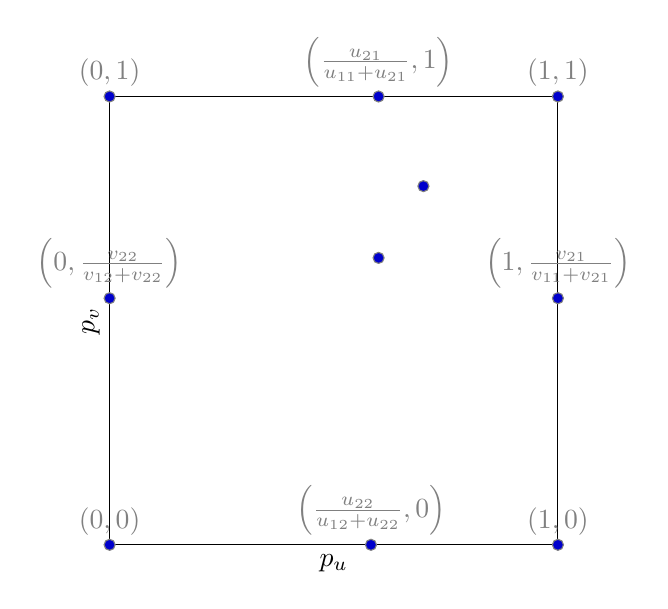
\begin{tikzpicture}
    \begin{axis}[xlabel=$\p_\pf$, ylabel=$\p_\pft$, unit vector ratio=1 1, xmin=0, xmax=1, ymin=0, ymax=1, xtickmin = -2, xtickmax =-1, ytickmin = -2, ytickmax =-1]
%            \draw [fill=qqqqff] (0.5,0.5) circle (2.5pt)
   \addplot+[nodes near coords, nodes near coords align={horizontal}, only marks, gray,
   point meta=explicit symbolic, gray]
table[meta=label] {
    x    y   label
    0  0 $(0,0)$
    1  0 $(1,0)$
    0  1 $(0,1)$
    1  1 $(1,1)$
    0  0.55  $\left(0,\frac{\pft_{22}}{\pft_{12} + \pft_{22}}\right)$
    0.583  0  $\left(\frac{\pf_{22}}{\pf_{12} + \pf_{22}},0\right)$
    1  0.55  $\left(1,\frac{\pft_{21}}{\pft_{11} + \pft_{21}}\right)$
    0.6  1  $\left(\frac{\pf_{21}}{\pf_{11} + \pf_{21}},1\right)$
    0.7  0.8  {}
    0.6  0.64  {}
};
    \end{axis}
    \end{tikzpicture}
\caption{The ten generic behavioral equilibria in a $2\times 2$ game. The two interior equilibria have long expressions that are not shown here.}
\label{genBeh}
\end{center}
\end{figure}







\begin{figure}[htb]
\begin{center}
\begin{tabular}{ccc}
& \begin{tabular}{|c|c|}
\hline
  \cellcolor{Turquoise}$C,C$ & \cellcolor{Turquoise}$C,D$ \\ \hline
\cellcolor{Turquoise}$D,C$ & \cellcolor{Turquoise}$D,D$\\ \hline
\end{tabular}
& \\
 & Outcome matrix & \\
 \\
\begin{tabular}{|c|c|}
\hline
  $\bn - \cs$ & $- \cs$ \\ \hline
$\frac{\bn - \cs}{\vh}$ & $\frac{\bn - \cs}{\vh}$ \\ \hline
\end{tabular} & \begin{tabular}{|c|c|}
\hline
  $\bn - \cs$ & $- \cs$ \\ \hline
$\bn$ & $0$ \\ \hline
\end{tabular}
& \begin{tabular}{|c|c|}
\hline
  $\bn - \frac{\cs}{2}$ & $\bn - \cs$ \\ \hline
$\bn$ & $0$ \\ \hline
\end{tabular} \\
Stag hunt & Prisoner's Dilemma & Snowdrift game \\

 & $\bn>\cs>0$, $\vh>1$ & \\
  
 \\
\end{tabular}
\\
\begin{tabular}{ccc}
\begin{tabular}{|c|c|}
\hline
  \cellcolor{LimeGreen}$+$ & \cellcolor{red}$-$ \\ \hline
\cellcolor{LimeGreen}$+$ & \cellcolor{white}$0$\\ \hline
\end{tabular}
 & \begin{tabular}{|c|c|}
\hline
  \cellcolor{LimeGreen}$+$ & \cellcolor{LimeGreen}$+$ \\ \hline
\cellcolor{red}$-$ & \cellcolor{red}$-$\\ \hline
\end{tabular}
\\
Realistic &  Other-regard\\
\\
\begin{tabular}{|c|c|}
\hline
  \cellcolor{red}$-$ & \cellcolor{red}$-$ \\ \hline
\cellcolor{LimeGreen}$+$ & \cellcolor{LimeGreen}$+$\\ \hline
\end{tabular}
 & \begin{tabular}{|c|c|}
\hline
  \cellcolor{LimeGreen}$+$ & \cellcolor{red}$-$ \\ \hline
\cellcolor{LimeGreen}$+$ & \cellcolor{red}$-$\\ \hline
\end{tabular} \\
 Selfish & Manipulator \\
\end{tabular}
\caption{The possible outcomes, the 3 different fitness games, and the 4 strategies considered in the discrete action model. A strategy is defined by the outcomes to which it associates a positive or negative utility in the corresponding outcome matrix (top). Cooperation is denoted by $C$ and defection by $D$. In the outcome matrix, the first letter refers to the action of the focal player (row) and the second letter to the action of its opponent (column). For example, the strategy Realistic associates a positive utility to the outcomes that yield positive material payoffs, and negative utility to outcomes yielding negative material payoffs. The strategy Other-regard associates a positive utility to the outcome where both the focal player cooperates ($C,\cdot$) and has a negative utility for outcomes where the focal player defects ($D,\cdot$).}
\label{stratDiscrete}
\end{center}
\end{figure}




\begin{figure}
%\vspace*{.05in}
\begin{center}
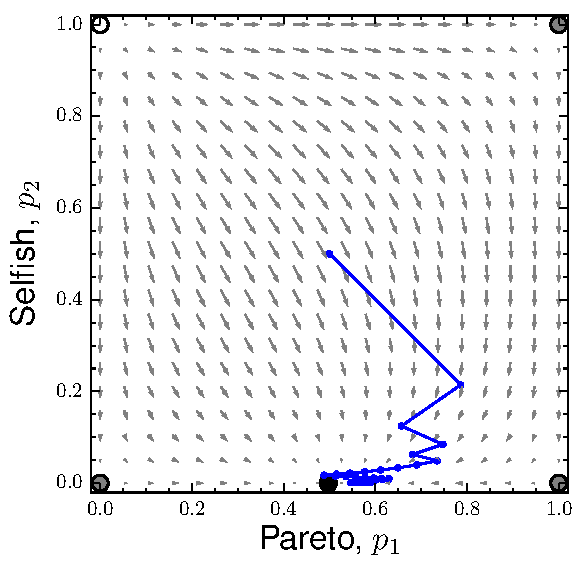
\includegraphics[scale=0.6]{DSps.pdf}
\caption{Vector field (gray arrows) and stochastic trajectory (blue line) for the interaction between ``Pareto'' and ``Selfish''. On the $x$-axis is represented the probability that Pareto cooperates ($p_1$), while on the $y$-axis, this is the probability that Selfish cooperates ($p_2$). The stochastic trajectory is started from the center of the state space $(p_1,p_2) = (\frac{1}{2},\frac{1}{2})$ and dots on it represent interaction rounds between the players. Circles represent equilibria: a white-filled circle is a source (both associated eigenvalues are positive); a gray-filled circle is a saddle (one positive and one negative associated eigenvalue); a black circle is a sink (both associated eigenvalues are negative).}
\label{cS}
\end{center}
\end{figure}


\begin{figure}
%\vspace*{.05in}
\begin{center}
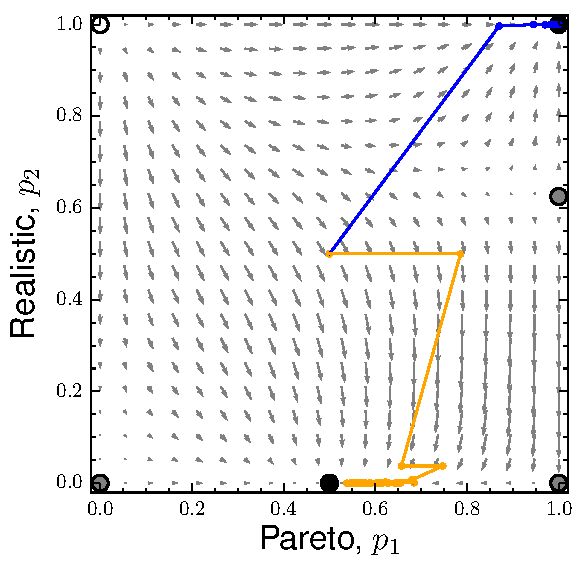
\includegraphics[scale=0.6]{DSpr.pdf}
\caption{Same as Fig.~\ref{cS} but for the interaction between Pareto and Realistic. Here the deterministic mean field equation admits two locally stable equilibria. The two stochastic trajectories of different color correspond to simulation runs that respectively converge to one of the locally stable equilibria.}
\label{dspr}
\end{center}
\end{figure}


\begin{figure}
%\vspace*{.05in}
\begin{center}
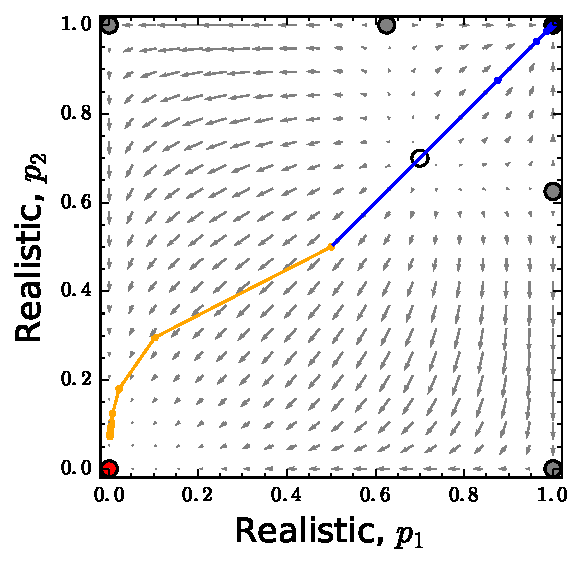
\includegraphics[scale=0.6]{DSrr.pdf}
\caption{Same as Fig.~\ref{cS} but for the interaction between Realistic and Realistic. The red-filled dot denotes an equilibrium with 0 eigenvalues.}
\label{dspr}
\end{center}
\end{figure}



\begin{figure}
%\vspace*{.05in}
\begin{center}
\includegraphics[scale=0.6]{dyn4strat.pdf}
\caption{Vector field for the replicator dynamics in the 4-strategy game defined by the competition between Realistic, Other-regard, Manipulator, and Selfish, when the underlying one-shot fitness game is a Prisoner's dilemma.}
\label{dspr}
\end{center}
\end{figure}






\begin{figure}[h]
\begin{center}
\begin{tabular}{l}
  (A) \\
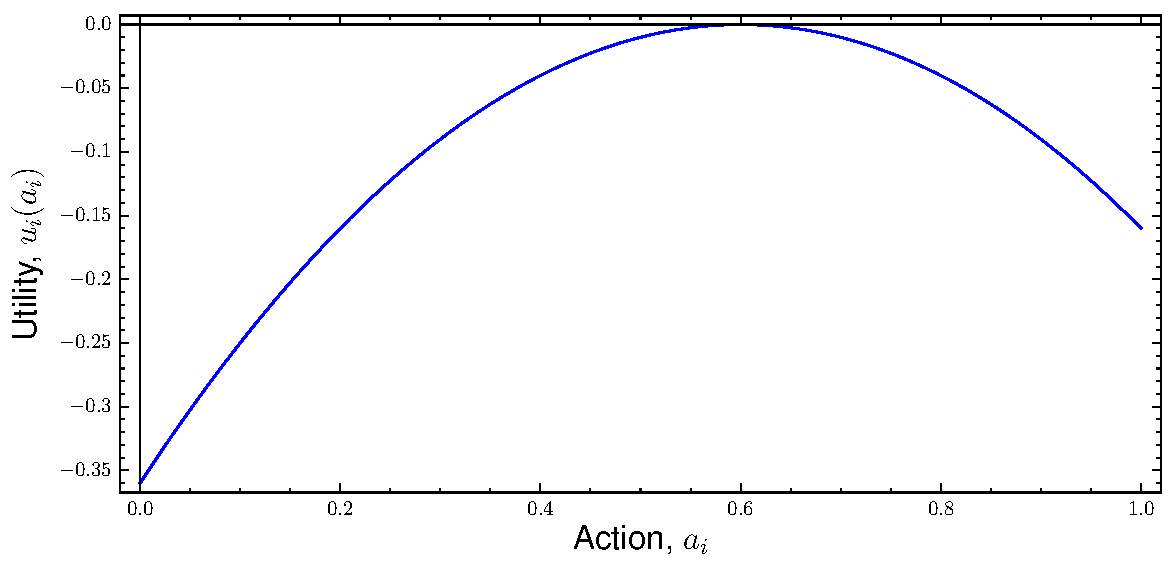
\includegraphics[scale=0.5]{simUf.pdf}\\
  (B) \\
 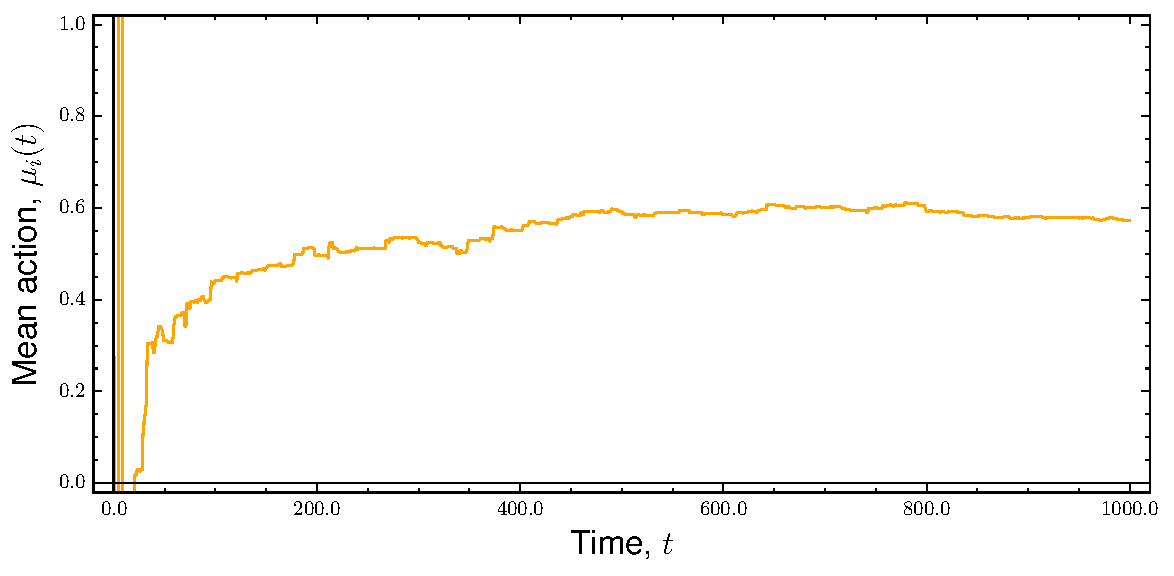
\includegraphics[scale=0.5]{meanDyn.pdf}\\
\end{tabular}
\caption{Continuous learning in a deterministic 1-player game. (A) The function $\pf_i(\ac_i)$ to be maximized by the player (eq.~\ref{cIndSim}), with $\ba=0.6$. (B) Typical dynamics of the mean action, $\ma_{i,\tm+1}$ when the utility function is that in (A).}
\label{simIndDyn}
\end{center}
\end{figure}






\end{document}
